\section{Adaptive Multi-Task Transfer Learning}\label{sec:multi-cws}

% As discussed in Section \ref{sec:intro}, CWS tools built on open source are not qualified for domain CWS tasks. The main reason is that supervised learning methods make the assumption that training data and test data are drawn from the same feature space, thus the performance drop is intuitively natural when there is a feature space drift. 

% However, in real world, it is common that we can learn a problem better and faster if we had learned another similar problem. %\KZ{Do you want to say
% % ``similar''? Your results show that the more disparity the better?} \GX{The overall improvement of transfer learning decreases when Disparity increases, considering the same target domain; but my approach gradually outperforms all baselines (relative improvement increases) when Disparity increases}
% % \GX{I assume you accept my explanation}
% For instance, learning French before may help to learn English. Similarly, learning to play the violin may help to accelerate learning the piano. Motivated by the intuition, people started to study the problem, named \textit{transfer learning}, since a NIPS-95 workshop, focused on machine-learning methods that retain and reuse previously learned knowledge, as reported by \newcite{Pan:2010:STL:1850483.1850545}.

With the motivation to leverage domain-invariant knowledge from high resource domain, we utilize the framework of multi-task learning ~\cite{Caruana1997}, which is one of the methods in \textit{transfer learning}, and further introduce three models under the proposed \textit{Adaptive Multi-Task Transfer Learning} framework (\textbf{AMTTL}). We exploit three statistical distance measures as the 
\textit{Adaptive} part to test the generality of our framework.

\subsection{Notations and Definitions}

% In this section, we introduce some notations and definitions that are used in later discussion. We define the multi-task learning in the context of our work.

In this paper, multi-task learning is defined as a \textit{dual-task} learning, which contains two \textit{domains} $\mathcal{D}_S$ and $\mathcal{D}_T$. Our purpose is to improve the performance of \textit{target domain} by exploiting knowledge from \textit{source domain}. 

Each domain $\mathcal{D}$ contains two components: a feature space $\mathcal{X}$ and a marginal probability distribution $P(X)$, where $X$ is a sample sentence,
and $X = \{x_1, \ldots, x_n\} \in \mathcal{X}$. 

% For example, if we treat CWS as a sequence tagging problem, then $\mathcal{X}$ is the space of all characters in training data. If two domains are different, e.g., news and medical, 
% they may have different feature spaces and different marginal probabilistic 
% distributions. 

Given a single domain, $\mathcal{D} = \{\mathcal{X}, P(X)\}$, a \textit{task} contains two components: a label space $\mathcal{Y}$ and a predictive function $f(\cdot)$, which can be learned during the training phase. Formally, $\mathcal{T} = \{\mathcal{Y}, f(\cdot)\}$.


\cut{%%%%%%%%%%%%%%%%%%%
\subsection{Statistical Distance}

In this section, we briefly introduce three statistical distance measures, Kullback–Leibler divergence, Maximum Mean Discrepancy, and Central Moment Discrepancy.

\subsubsection{Kullback–Leibler divergence}
{\em Kullback–Leibler divergence} (KL), is a non-symmetric measure of the divergence between two distributions. For two discrete probability distributions $P$ and $Q$, the KL divergence from $Q$ to $P$ is defined as:

\small
\begin{equation}
D_{KL}(P||Q) = \sum_i{P(i)\log{\frac{P(i)}{Q(i)}}}
\end{equation}
\normalsize

the Kullback–Leibler divergence between $P$ and $Q$ is defined as:

{\small
\begin{equation}
\textnormal{KL}(P, Q) = D_{KL}(P||Q) + D_{KL}(Q||P)
\end{equation}
}

\subsubsection{Maximum Mean Discrepancy}
Proposed by \newcite{Gretton:2012:KTT:2188385.2188410}, 
{\em maximum mean discrepancy} (MMD) is a nonparametric statistical 
test used to determine if two samples are drawn from different distribution.  
Given two sets of samples $X = \{x_i, \ldots, x_m\}$ and 
$Y = \{y_1, \ldots, y_n\}$, the empirical estimate of MMD is defined as 
the distance between the empirical mean embedding of each distribution:

% The test statistic is the largest difference in expectations over functions in the unit ball of a reproducing kernel Hilbert space $\mathcal{H}$ (RKHS). 
% Given two distribution $p$ and $q$, and a class of functions $\mathcal{F} = \{f : \mathcal{X} \rightarrow \mathbb{R}\}$, MMD is defined as 

% \small
% \begin{equation}
% % \setlength{\abovedisplayskip}{0pt}
% % \setlength{\belowdisplayskip}{0pt}
% \textnormal{MMD}[\mathcal{F}, p, q] := \sup_{f\in \mathcal{F}}(\mathbb{E}_x[f(x)] - \mathbb{E}_y[f(y)])
% \end{equation}
% \normalsize

 % Consider $\mathcal{F}$ as the unit ball in reproducing kernel Hilbert space $\mathcal{H}$, it is proven that $\textnormal{MMD}[\mathcal{F}, p, q] = 0$ \textit{iff.} $p = q$. 
\begin{equation}
 \small
% \setlength{\abovedisplayskip}{0pt}
% \setlength{\belowdisplayskip}{0pt}
\textnormal{MMD}^2[\mathcal{F}, p, q] := \left|\left|\frac{1}{m}\sum_{i=1}^m\phi(x_i) - \frac{1}{n}\sum_{i=1}^n\phi(y_i)\right|\right|_\mathcal{H}
\end{equation}
where $\mathcal{F}$ is the unit ball in reproducing kernel Hilbert space $\mathcal{H}$.

\subsubsection{Central Moment Discrepancy}

Proposed by ~\cite{DBLP:journals/corr/ZellingerGLNS17}, {\em Central Moment Discrepancy} (CMD) is a new distance function on probability distributions on compact intervals. Let $X$ and $Y$ be bounded random samples with respective probability distributions $p$ and $q$ on the interval $[a, b]^N$. The central moment discrepancy $\textnormal{CMD}_K$ is defined as an empirical estimate of the CMD metric:
% Two theorems that identify CMD as a metric and analyze a convergence property are also proven in ~\cite{DBLP:journals/corr/ZellingerGLNS17}. The final CMD loss is defined as an empirical estimate of CMD.
\begin{equation}
\small
\begin{aligned}
\textnormal{CMD}_K(X, Y) &= \frac{1}{|b-a|}||\textnormal{\textbf{E}}(X)-\textnormal{\textbf{E}}(Y)||_2 \\&+ \sum_{k=2}^K{\frac{1}{|b-a|^k}}||C_k(X)-C_k(Y)||_2
\end{aligned}
\end{equation}
where $\textnormal{\textbf{E}}(X) = \frac{1}{|X|}\sum_{x\in X}x$ is the empirical expectation vector computed on the sample $X$ and $C_k(X) = \textnormal{\textbf{E}}((x - \textnormal{\textbf{E}}(X))^k)$ is the vector of all $k_{th}$ order sample central moments of the coordinates of $X$. In experiment, we set $K$ to $5$, following ~\cite{DBLP:journals/corr/ZellingerGLNS17}.

}%%%%%%%%%%%%%%%%%end of cut %%%%%%%%%%%%%%

\subsection{Formal Definition}
We now give the definition of \textit{Adaptive Multi-Task Transfer Learning}.

\theoremstyle{definition}
\begin{definition}
Given two domains $\mathcal{D}_S$ and $\mathcal{D}_T$, and corresponding tasks $\mathcal{T}_S$, $\mathcal{T}_T$, \textit{Adaptive Multi-Task Transfer Learning} aims to improve the learning of target predictive function $f_T(\cdot)$ by using \textit{shared parameter} and \textit{minimizing the distance} between $P(X_S)$ and $P(X_S)$, $P(Y_S|X_S)$ and $P(Y_T|X_T)$, where $\mathcal{D}_S \neq \mathcal{D}_T$, or $\mathcal{T}_S \neq \mathcal{T}_T$.
\end{definition}

\subsection{Objective Function}\label{sec:objective}

The objective function of our proposed \textit{Adaptive Multi-Task Transfer Learning} can be formulated as follows:

\small
\begin{equation}\label{eq:objective}
\mathcal{J}(\theta^{(a)}, \theta^{(b)}) = \mathcal{J}_{seg} + \alpha\mathcal{J}_{Adap.} + \beta\mathcal{J}_{L_2}
\end{equation}
\normalsize
where $\theta^{(a)}$ and $\theta^{(b)}$ are model parameters for task $a$ and $b$, $\alpha$ and $\beta$ are hyper-parameters to be chosen.

$\mathcal{J}_{seg}$ stands for the negative log likelihood for source domain and target domain. At each training step, we minimize the mean negative log likelihood:

\small
\begin{equation}
\begin{aligned}
\mathcal{J}_{seg} = -\frac{1}{n}\sum_{i=1}^n\log p(Y_i^{(a)}|X_i^{(a)}) \\ -\frac{1}{m}\sum_{i=1}^m\log p(Y_i^{(b)}|X_i^{(b)})
\end{aligned}
\end{equation}
\normalsize

$\mathcal{J}_{Adap.}$ is the \textit{Adaptive} loss used to capture domain-invariant knowledge between different domains, which forces the hidden representations between two domains to \textit{adapt} to each other. Given two sets of hidden representation, denoted as $\mathbf{h^{(a)}}$ and $\mathbf{h^{(b)}}$, and a statistic distance function $g(\cdot)$, $\mathcal{J}_{\textnormal{Adap.}}$ can be calculated as:

\small
\begin{equation}\label{eq:Adap}
\mathcal{J}_{\textnormal{Adap.}} = g(\mathbf{h^{(a)}}, \mathbf{h^{(b)}})
\end{equation}
\normalsize

\noindent where $g(\cdot)$ can be, but is not limited to, 
KL divergence, maximum mean discrepancy 
(MMD)~\cite{Gretton:2012:KTT:2188385.2188410} or central moment discrepancy 
(CMD)~\cite{DBLP:journals/corr/ZellingerGLNS17}; $\mathbf{h^{(a)}}$ and $\mathbf{h^{(b)}}$ are different for different model setting, which will be defined in Sec \ref{sec:models}.

$\mathcal{J}_{L_2}$ is the $L_2$ regularization which is used to control overfitting problem:
\small
\begin{equation}
\mathcal{J}_{L_2} = \left|\left|\theta^{(a)}\right|\right|^2_2 + \left|\left|\theta^{(b)}\right|\right|^2_2
\end{equation}
\normalsize

\subsection{Models}\label{sec:models}

% To exploit different settings of shared layer, domain-specific layer and \textit{Adaptive loss}, we propose three models for cross-domain CWS task as shown in Figure \ref{fig:model}.

In this section, we present the design of three variants of our framework in detail. The architectures are presented in Figure \ref{fig:model}.

\begin{figure*}[ht!]
\begin{subfigure}{.33\textwidth}
% 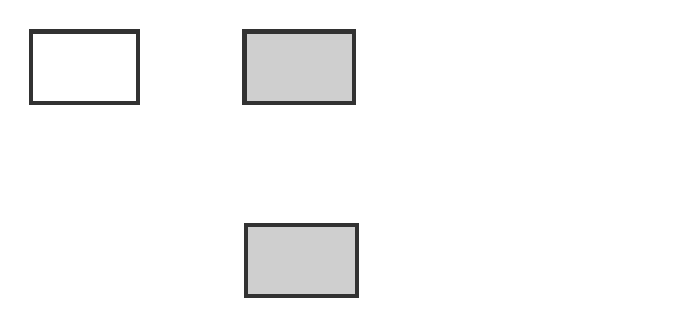
\includegraphics[width=\textwidth]{assets/model_1.png}
\def\svgwidth{\textwidth}
\input{assets/model_1.pdf_tex}
\caption{Model-\RN{1}}\label{fig:model_1}
\end{subfigure}
\begin{subfigure}{.33\textwidth}
% 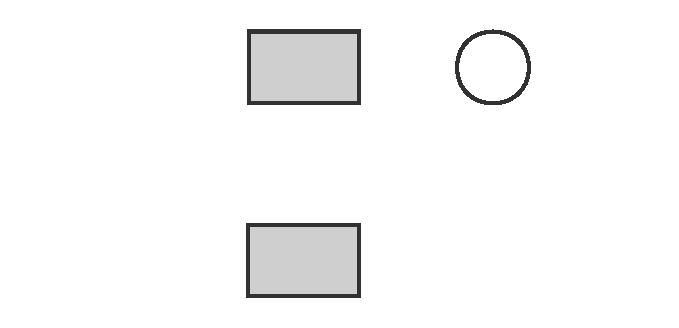
\includegraphics[width=\textwidth]{assets/model_2.png}
\def\svgwidth{\textwidth}
\input{assets/model_2.pdf_tex}
\caption{Model-\RN{2}}\label{fig:model_2}
\end{subfigure}
\begin{subfigure}{.33\textwidth}
% 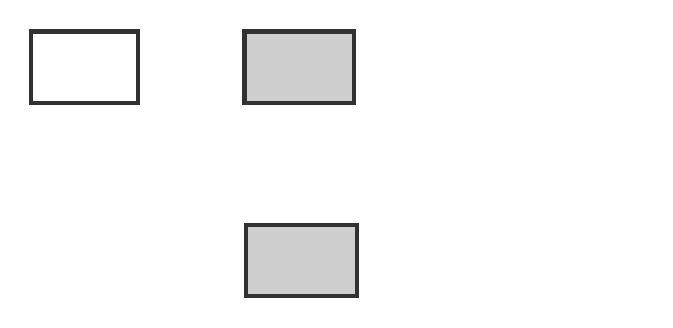
\includegraphics[width=\textwidth]{assets/model_3.png}
\def\svgwidth{\textwidth}
\input{assets/model_3.pdf_tex}
\caption{Model-\RN{3}}\label{fig:model_3}
\end{subfigure}
\caption{Three models with different settings. The white block represents Embedding lookup layer, while the gray and black block represents Bi-LSTM layer. The ``SHARED'' in Figure \ref{fig:model_2} stands for shared Bi-LSTM for both tasks. The ``$\mathcal{J}_\textnormal{Adap.}$'' represents \textit{Adaptive} loss for the hidden representation after corresponding layer, which is formally discussed in Sec \ref{sec:objective}. The solid arrow and dotted arrow show the flow of task $a$ and task $b$ respectively.}\label{fig:model}
\end{figure*}

\subsubsection{Model-\RN{1} Specific LSTM}

This model can be interpreted as two \textit{parallel tasks} connected with $\mathcal{J}_{\textnormal{Adap.}}$ after specific Bi-LSTM layers of two tasks. We design the model in order to see whether knowledge can actually be transfered through the \textit{Adaptive} loss alone.

The hidden representation and CRF score of \textit{task} $t$ at position $i$ can be computed as:

\small
\begin{equation}\label{eq:model_1_h}
h_i^{(t)} = \textnormal{Bi-LSTM}(X^{(t)}, \theta^{(t)})
\end{equation}
\begin{equation}\label{eq:model_1_s}
s(X, i)^{(t)} = \mathbf{W^{(t)}}^\top h_i^{(t)} + \mathbf{b}^{(t)}
\end{equation}
\normalsize

\noindent where $h_i^{(t)} \in \mathbb{R}^{2d_h}$, $\mathbf{W^{(t)}} \in \mathbb{R}^{2d_h \times |\mathcal{L}|}$, $\mathbf{b}^{(t)} \in \mathbb{R}^{|\mathcal{L}|}$, $\theta^{(t)}$ denotes parameters of domain specific Bi-LSTM. The $\mathcal{J}_{\textnormal{Adap.}}$ between two tasks, denoted by $a$ and $b$, is formulated as:

\small
\begin{equation}\label{eq:model_1_adap}
\mathcal{J}_{\textnormal{Adap.}} = g(\mathbf{h}^{(a)}, \mathbf{h}^{(b)})
\end{equation}
\normalsize

\noindent where $\mathbf{h}^{(t)} = \{h_i^{(t)} | X^{(t)} \in \mathcal{X}^{(t)}\}$, $\mathcal{X}^{(t)}$ is a batch of input sequences.

\subsubsection{Model-\RN{2} Shared LSTM}

Model-\RN{2} is designed to adopt domain specific embedding layers, shared 
Bi-LSTM layer and domain specific CRF layers. Note that traditional 
\textit{multi-task learning} uses shared embedding~\cite{DBLP:journals/corr/Ruder17a}. 
Shared embedding means that source and target domain share the same set of 
embedding parameters while domain-specific embedding means that the two 
domains maintain their own sets.
% Unlike traditional ways of sharing low-level layers ~\cite{DBLP:journals/corr/Ruder17a}, we adopt specific embedding layer for each task. The \textit{heterology} of embedding space shouldn't be forced by sharing word embeddings. 

The hidden representation of \textit{task} $t$ at position $i$ can be 
computed as:

\small
\begin{equation}\label{eq:model_2_h}
h_i^{(t)} = \textnormal{Bi-LSTM}(X^{(t)}, \theta)
\end{equation}
\normalsize
\noindent where two tasks share Bi-LSTM parameter $\theta$, which is the only 
difference with Model-\RN{1}. CRF score and $\mathcal{J}_{\textnormal{Adap.}}$ 
is the same as \eqref{eq:model_1_s}\eqref{eq:model_1_adap}.

\subsubsection{Model-\RN{3} Shared \& Specific LSTM}

Model-\RN{3} is a combination of Model-\RN{1} and Model-\RN{2}, 
with both domain specific and shared Bi-LSTM layers.

The hidden representation and CRF score of \textit{task} $t$ at position 
$i$ can be computed as:

\begin{equation}
\small
\begin{aligned}
h_i^{(t)} &= \textnormal{Bi-LSTM}(X, \theta^{(t)}) \oplus \textnormal{Bi-LSTM}(X, \theta)\\
&= h_{i(specific)}^{(t)} \oplus h_{i(shared)}^{(t)}
\end{aligned}
\end{equation}
\begin{equation}
s(X, i)^{(t)} = \mathbf{W^{(t)}}^\top h_i^{(t)} + \mathbf{b}^{(t)}
\end{equation}

\noindent where $h_i^{(t)} \in \mathbb{R}^{4d_h}$, $\mathbf{W^{(t)}} \in \mathbb{R}^{4d_h \times |\mathcal{L}|}$, and $\mathbf{b}^{(t)} \in \mathbb{R}^{|\mathcal{L}|}$. $\theta^{(t)}$ and $\theta$ denote the parameter of domain specific and shared Bi-LSTM. $\mathcal{J}_{\textnormal{Adap.}}$ can be calculated as :

\begin{equation}
\small
\mathcal{J}_{\textnormal{Adap.}} = g(\mathbf{h}^{(a)}, \mathbf{h}^{(b)})
\end{equation}

\noindent where $\mathbf{h}^{(t)} = \{h_{i(specific)}^{(t)} | X^{(t)} \in \mathcal{X}^{(t)}\}$, $\mathcal{X}^{(t)}$ is a batch of input sequences.

